\chapter{Simulation}
\label{sec:simulation}
Im diesem Kapitel wird die Simulation anhand von MATLAB/Simulink (Version R2018a) dargestellt. Dabei werden die Fahrparameter dynamisch berechnet. Um dies zu erreichen wurde das Modell für den Differentialantrieb aufgebaut, um Vorhersagen über das Fahrverhalten treffen zu können. 
Die modellbasierte Simulation erlaubt es Fahrdynamikregelsysteme zu entwickeln, ohne teure Tests unternehmen zu müssen. Abbildung 4.1 verdeutlicht den Unterschied der in diesem Kapitel vorgestellten Regelungsarten, die beide in unserem Modell gebraucht werden.

\begin{figure}[htb]
  \centering  
  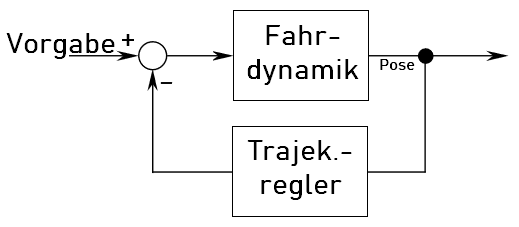
\includegraphics[scale=2]{img/vier.png}
  \caption{Zusammenwirken des Dynamischen Reglers (Kapitel 4.1) und des Trajektorien Reglers (Kapitel 4.2)}
  \label{fig:Zusammenwirken des Dynamischen Reglers (Kapitel 4.1) und des Trajektorien Reglers (Kapitel 4.2)}
\end{figure} 


\section{Dynamische Regelung}
Abbildung 4.2 zeigt das einfachere Fahrzeugmodell im Blockschaltbild samt Regler. In dem oberen Kasten erfolgt die Berechnung der Geschwindigkeit und der Winkelgeschwindigkeit aus den beiden Radgeschwindigkeiten. Als Ausgabe erhält man die aktuellen Werte, die in dem Regler mit den Soll-Werten aus der Trajektorie verglichen werden. Aus Gründen der Übersichtlichkeit übernimmt der Regler zusätzlich die Aufgabe des Umrechnens der Regelgrößen. Als Ergebnis bekommt man also die Stellgrößen für die Geschwindigkeit der beiden Räder heraus, die an die Aktuatoren weitergegeben werden. Im nun folgenden Modell nehmen wir jedoch nicht die beiden Radgeschwindigkeiten als input, sondern die lineare- und Winkelgeschwindigkeit. \\
\begin{figure}[htb]
  \centering  
  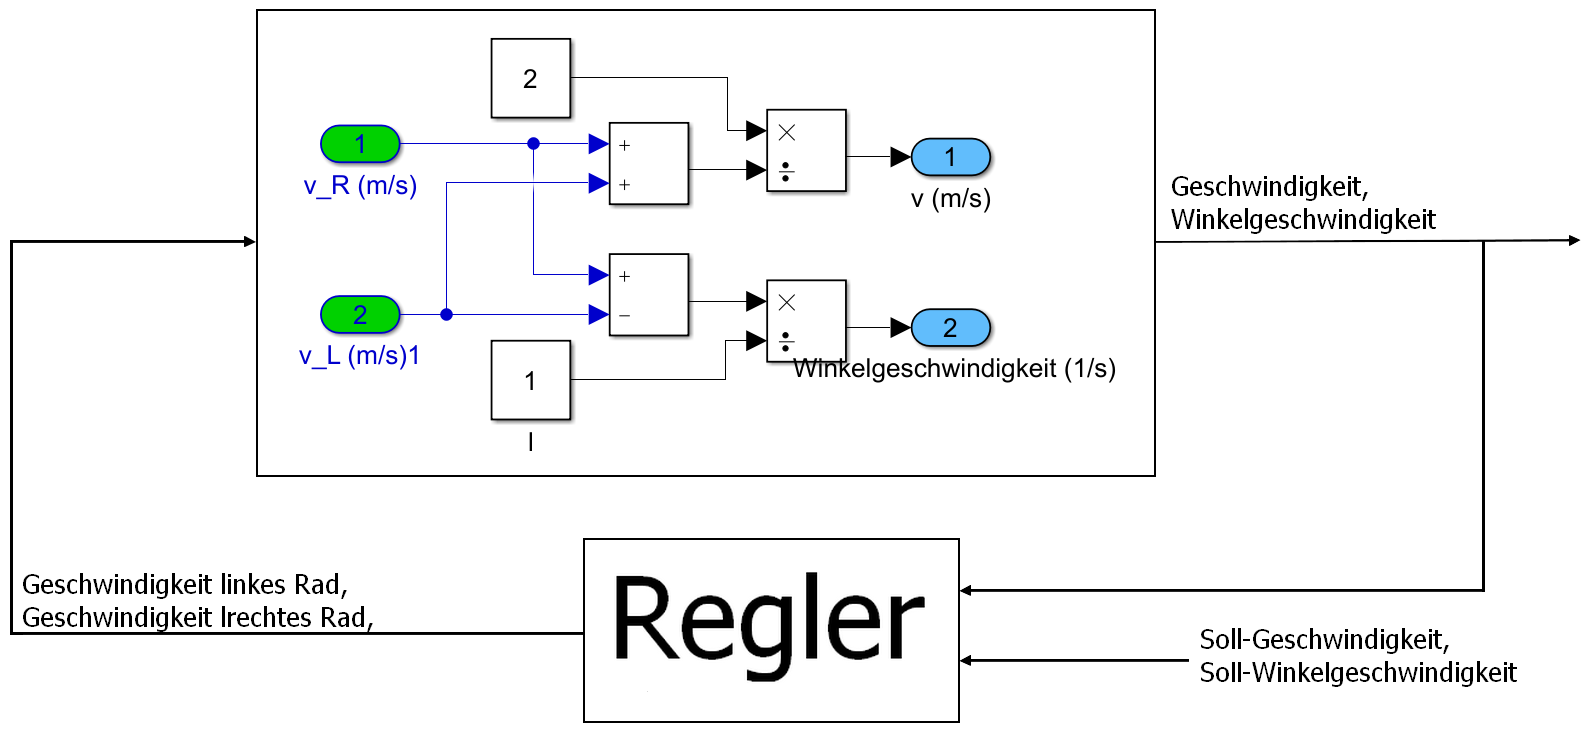
\includegraphics[scale=1]{img/Blockschaltbild1.png}
  \caption{Logischer Aufbau unseres Modells}
  \label{fig:starwars}
\end{figure}
Mithilfe von Simulink lässt sich eine Simulation erstellen, anhand derer man sich vergewissern kann, dass das in Kapilel 3 erstellte mathematische Modell tatsächlich so funktioniert, wie erwartet. Abbildung 4.3 zeigt das zur Simulation dazugehörige Blockschaltbild. Als Eingabe wird die (Tangenten-)Geschwindigkeit und die Winkelgeschwindigkeit bestimmt. Durch die inverse Kinematik werden anhand dieser Eingangsgrößen die Geschwindigkeiten beider Räder berechnet, die selbst schon ein Ausgangssignal bilden (Pfeil nach unten). Folgt man dem Pfeil nach oben, so wird aus den beiden Radgeschwindigkeiten wieder in Geschwindigkeit und Winkelgeschwindigkeit transformiert, mittels direkter Kinematik. Bei dem mittleren Pfeil wird aus den Radgeschwindigkeiten die Pose des Fahrzeugs ermittelt. \\
An den beiden Reglern lassen sich die Eingangsgrößen Geschwindigkeit und Winkelgeschwindigkeit verstellen, was sich unmittelbar in der Simulation auswirkt, sodass man sofort eine visuelle Rückmeldung für die veränderten Größen bekommt. Ändert man die Werte nicht, so bleibt die Geschwindigkeit und die Tangentengeschwindigkeit konstant, was eine Kreisbewegung des Fahrzeugs zur Folge hat (für $\omega \not= 0$). Da an dieser Stelle noch keine vorgegebene Trajektorie abgefahren werden soll, gibt es auch keinen Regler.
\begin{figure}[htb]
  \centering  
  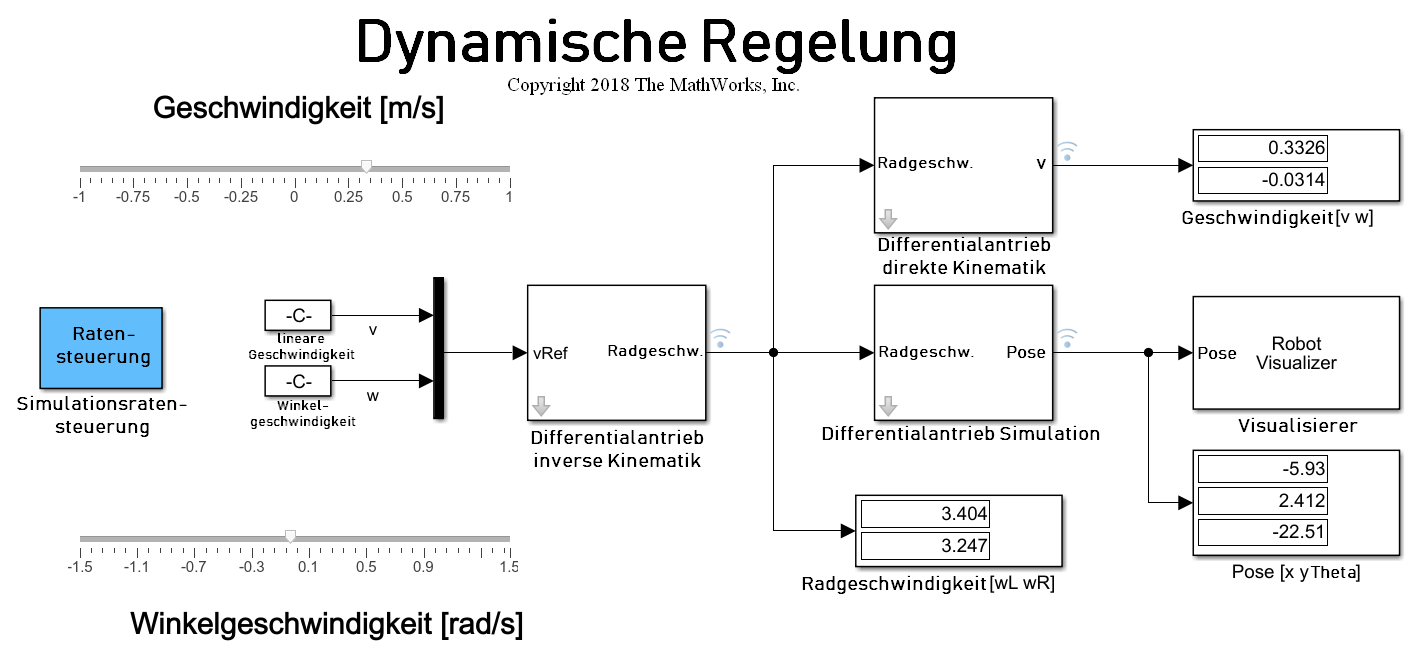
\includegraphics[scale=1.4]{img/simulation1.png}
  \caption{Simulation - Blockschaltbild einfaches Modell}
  \label{fig:starwars}
\end{figure}
Als Beispiel für das Ergebnis dieser Simulation, ist in Abbildung 4.5 eine selbsterklärende Momentaufnahme zu sehen. Die Abstände der einzelnen Punkte zueinander geben Hinweise auf die aktuelle Geschwindigkeit, und die Kreisbahn ist abhängig von der gewählten Winkelgeschwindigkeit. \\
\begin{figure}[H]
  \centering  
  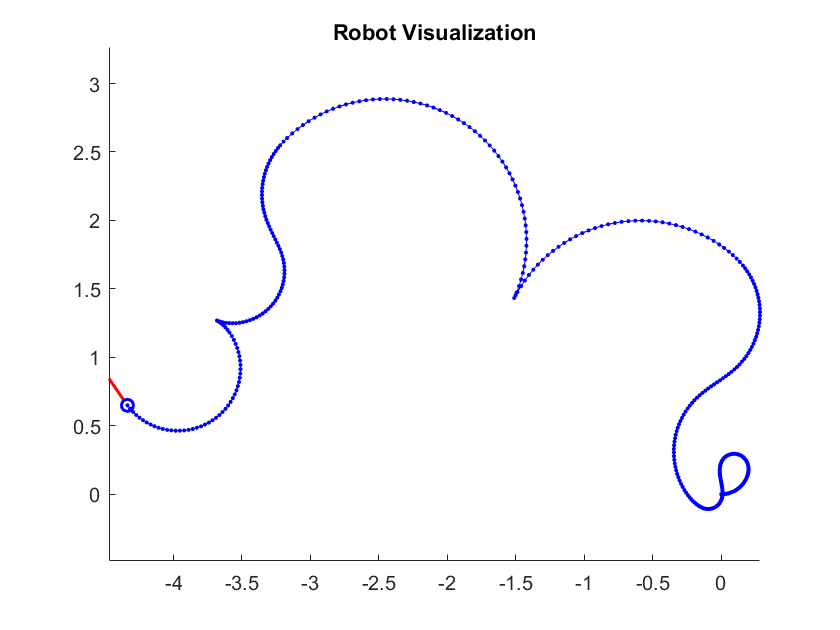
\includegraphics[scale=0.7]{img/simulationsergebnis2.png}
  \caption{Simulation - Ergebnis der Simulation der Kinematik}
  \label{fig:starwars}
\end{figure}

\section{Trajektorien Regelung}
Ein weiteres Blockschaltbild (Abbildung 4.5) simuliert das Verhalten des gleichen Fahrzeugs beim Abfahren verschiedener vorgegebener Punkte mittels Regler, sprich der Trajektorienregelung. Das Ergebnis wird in Abbildung 4.6 veranschaulicht. Die leichten Abweichungen liegen an der Regelung und an dem gewählten Maximalabstand, ab dem ein Zielpunkt als erreicht gilt.
\begin{figure}[htb]
  \centering  
  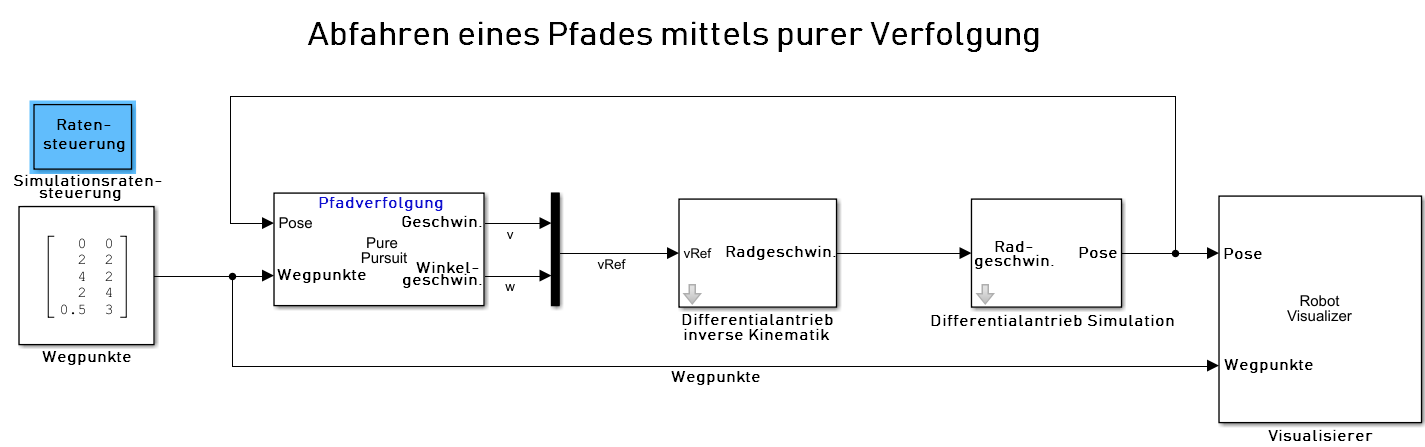
\includegraphics[scale=1.4]{img/einfachesmodellpunkteanfahrensimulation.png}
  \caption{Simulation - Vorgegebene Koordinaten abfahren}
  \label{fig:starwars}
\end{figure}

In dieser Simulation soll ein möglichst kurzer Pfad zwischen aktueller Position des Fahrzeugs und dem Ziel bestimmt werden. Möglichst kurz ist hier gleichzusetzen mit möglichst wenig Lenkung, was zu einer 'geraderen' Strecke führt. \\
Anders als bei vorherigen Simulation, spielen hier auch die Trajektorienplanung und die dynamische Regelung entscheidende Rollen. \\
Da man nur ein paar abzufahrende Punkte hat und nicht etwa eine alles verbindende Streckenvorgabe, muss der Pfad bestimmt werden bevor sich das Fahrzeug in Bewegung setzt.  

\begin{figure}[H]
  \centering  
  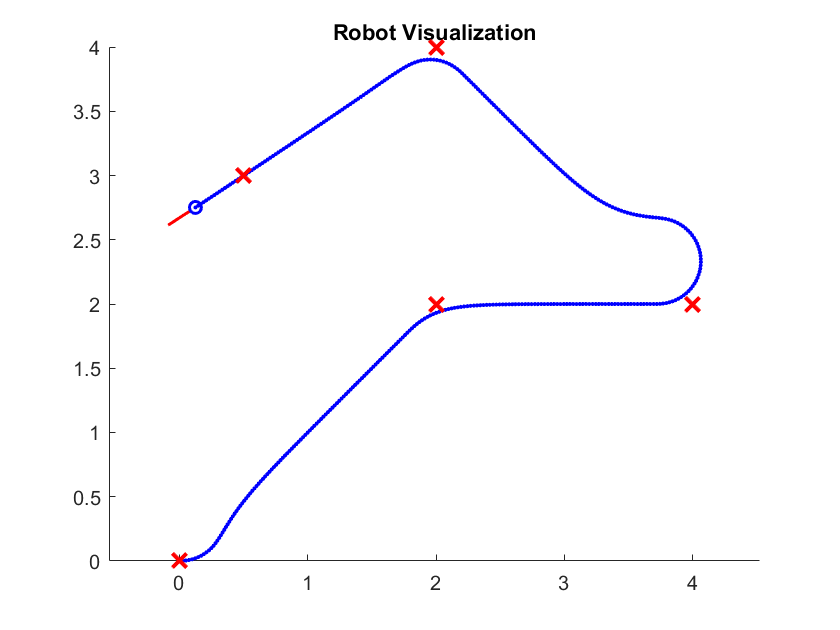
\includegraphics[scale=0.7]{img/simulationsergebnis1.png}
  \caption{Simulation - Ergebnis Punkte abfahren}
  \label{fig:starwars}
\end{figure}

Im folgendem Kapitel wird mittels Raspberry Pi ein Prototyp realisiert. Dies geschieht über die Software-Hardware-Schnittstelle, die das digitale Ansteuern von Analogen Aktuatoren ermöglicht.




